% Experiment results
The experiment results of Hockney model is shown as below. We estimated the running time for different number of MPI ranks. Figure 1 shows the comparison between them.

For this experiment, the message size chanegs from 1 to 1024 by the power of two.
And the rank number per node changes from 1 to 6 for up to two nodes.
After the testing in different conditioins, it is found that the lantency of the network is almost static which is fixed around 0.004 ms.

\begin{figure*}[h]
\centering
\hspace*{\fill}
\subfloat[Rank 1]{
  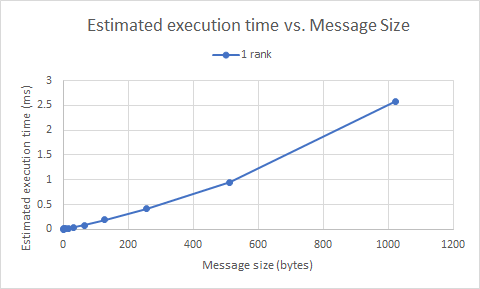
\includegraphics[width=0.45\linewidth]{exe_time_vs_messsage_size_rank_1.png}
}
\hspace*{\fill}
\subfloat[Rank 2]{
  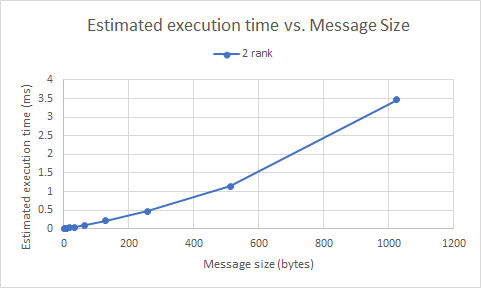
\includegraphics[width=0.45\linewidth]{exe_time_vs_messsage_size_rank_2.png}
}
\hspace{0mm}
\subfloat[Rank 3]{
  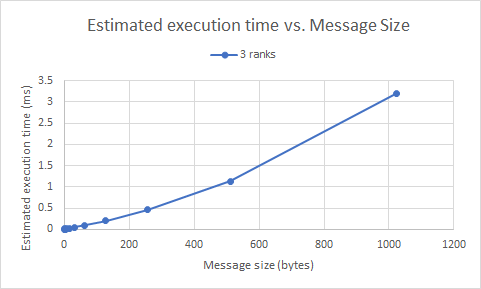
\includegraphics[width=0.4\linewidth]{exe_time_vs_messsage_size_rank_3.png}
}
\hspace*{\fill}
\subfloat[Rank 4]{
  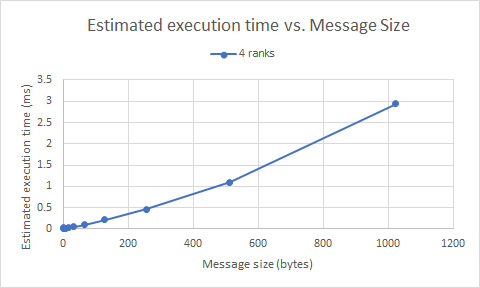
\includegraphics[width=0.45\linewidth]{exe_time_vs_messsage_size_rank_4.png}
}
\hspace{0mm}
\subfloat[Rank 5]{
  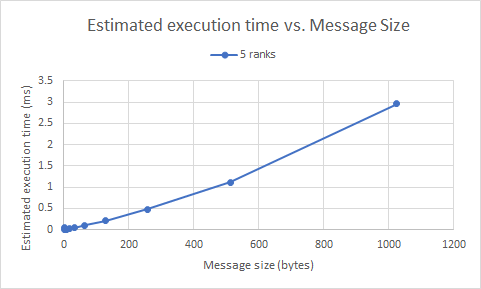
\includegraphics[width=0.45\linewidth]{exe_time_vs_messsage_size_rank_5.png}
}
\hspace*{\fill}
\subfloat[Rank 6]{
  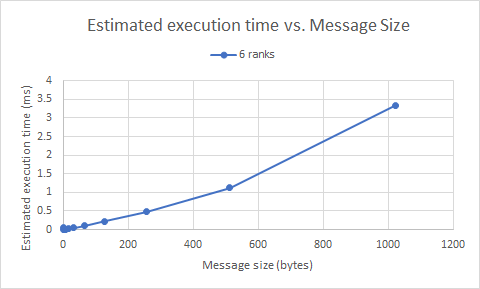
\includegraphics[width=0.45\linewidth]{exe_time_vs_messsage_size_rank_6.png}
}
\caption{Estimated execution time vs message size along different ranks.}
\end{figure*}

Figure 2 shows the result comparison of estimated execution time across different ranks versus message size and number of ranks. Note that the green column in Figure 2(b) represents the result from running on 2 nodes with each nodes having 6 MPI ranks.

\begin{figure*}[h!]
\hspace{0mm}
\subfloat[Comparison of estimated execution time vs message size across different ranks.]{
	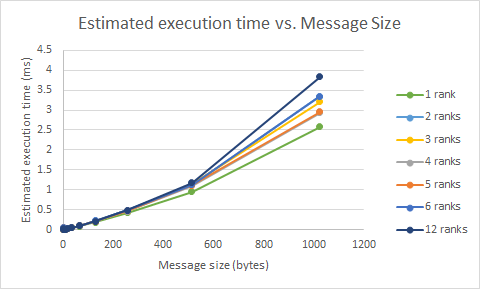
\includegraphics[width=0.5\linewidth]{estimated_execution_time_vs_message_size.png}
}
\hspace*{\fill}
\subfloat[Estimated execution time in relation to ranks]{
	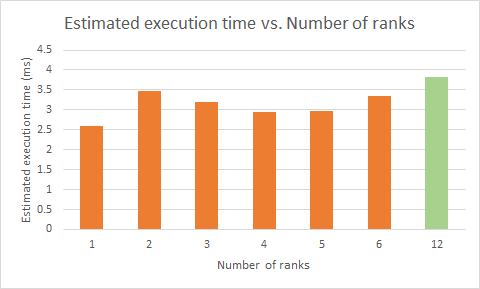
\includegraphics[width=0.5\linewidth]{estimated_execution_time_vs_number_of_ranks_1.png}
}
\caption{The relationship between message sizes and number of ranks to estimated execution time.}
\end{figure*}


\begin{figure}[h]
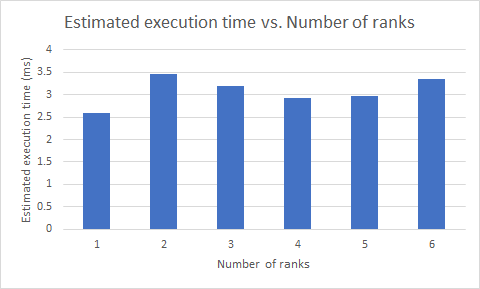
\includegraphics[width=0.5\textwidth]{estimated_execution_time_vs_number_of_ranks.png}
\caption{An alternative interpretation of the relations between estimated execution time and the number of ranks.}
\end{figure}